\documentclass{ctexart}%%中文文档类型
\usepackage{graphicx}%%插图宏包
\usepackage{float}%%固定图片位置,使用参数H

%%并排放两张图片的包
\usepackage{subfig}%多个子图
\usepackage{caption}%注释设置

% Windows系统使用
\usepackage{xeCJK}
\setCJKmainfont{SimSun}
\begin{document}
% Mac系统使用
%\usepackage{xeCJK}
%\setCJKmainfont[BoldFont=STHeiti,ItalicFont=STKaiti]{STSong}
%\setCJKsansfont[BoldFont=STHeiti]{STXihei}
%\setCJKmonofont{STFangsong}	



%%单张图片插入
\begin{figure}[!htb]
	%其中!h只是试图将图片放在当前位置,如果页面剩下的部分放不下,还是会跑到下一页的(t)顶部或者(b)底部。
	%H借助float包可以固定图片位置
	\centering
	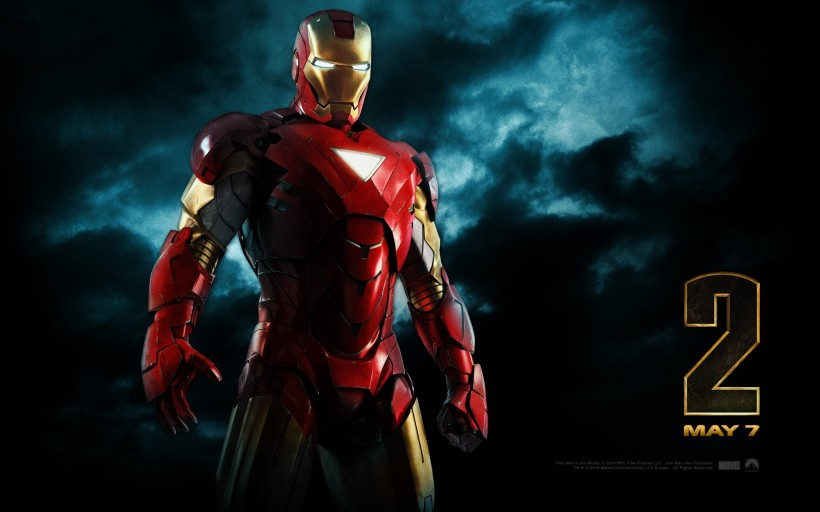
\includegraphics[width = 0.7\linewidth]{./pictures/1.jpg}
	\caption{钢铁侠}\label{fig:1}
\end{figure}


%并排两张图片插入
\begin{figure}[htbp]  %[htbp]中的h是浮动的意思
	\centering    %居中
	\subfloat[钢铁侠] %第一张子图
	{	\begin{minipage}[t]{0.5\textwidth}
			\centering  %子图居中
			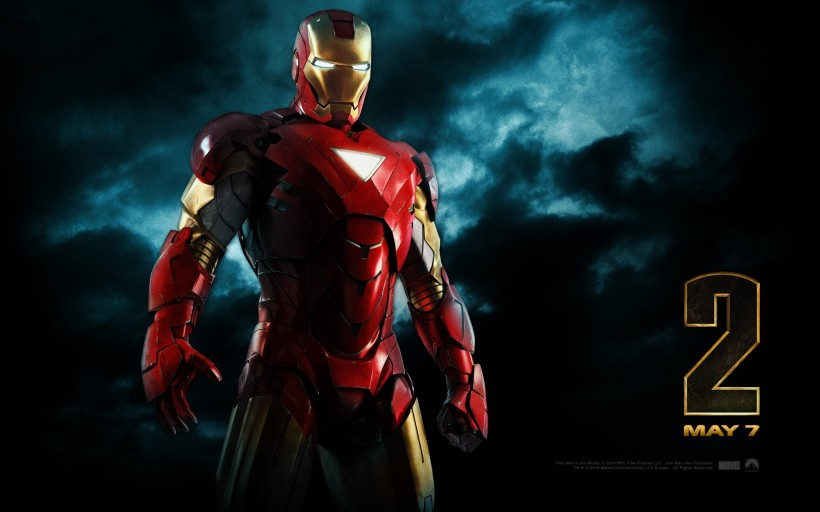
\includegraphics[width=0.65\textwidth]{./pictures/1.jpg}   %以行宽的0.5倍大小显示
			\label{fig1}
		\end{minipage}%
	}%注意这里不能回车空行,否则两张图会上下排列,而不是并排排列
	\subfloat[黑寡妇] %第二张子图
	{	\begin{minipage}[t]{0.5\textwidth}
			\centering %子图居中
			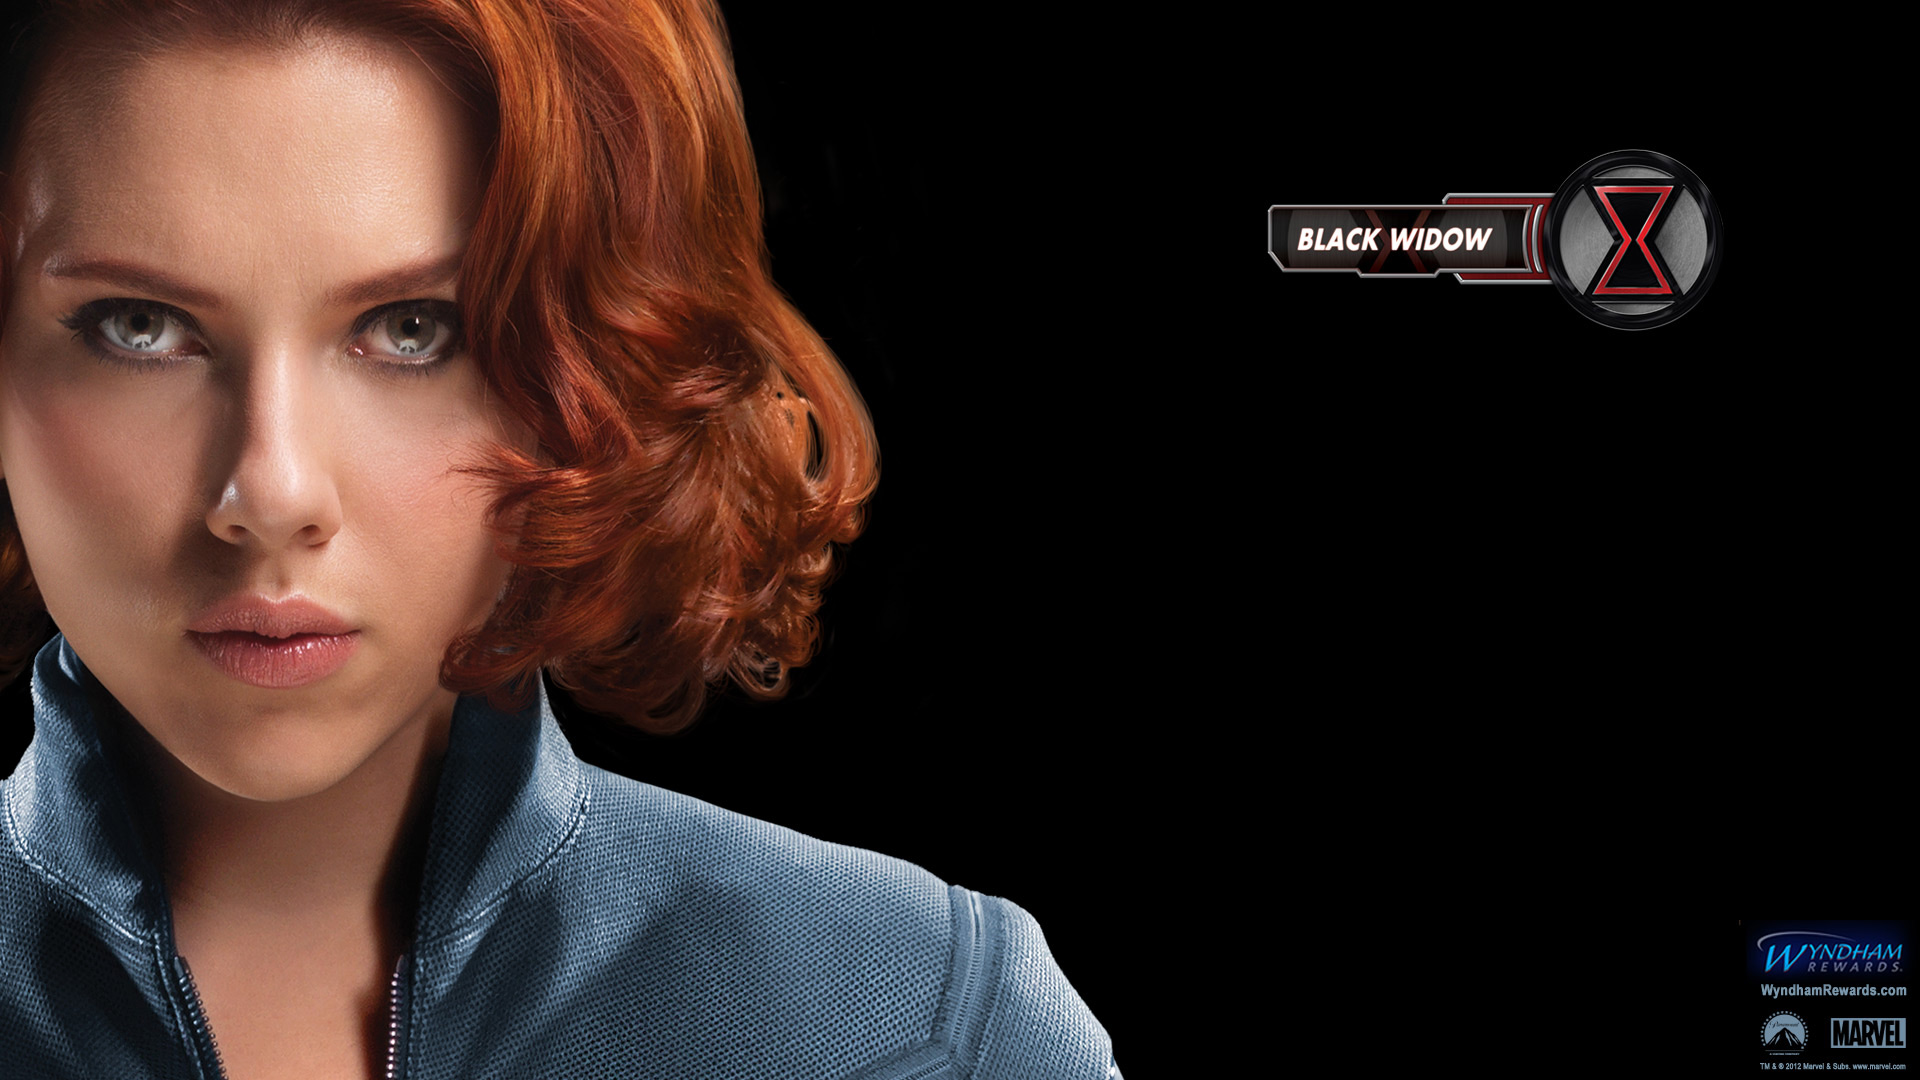
\includegraphics[width=0.65\textwidth]{./pictures/2.jpg}   %以行宽的0.5倍大小显示
			\label{fig2}
		\end{minipage}
	}
	\caption{复仇者联盟} %  %大图名称
	\label{FIG}  %图片引用标记
\end{figure}


%% 插入2*2排列图片,m*n类似,用 \quad 来换行
\begin{figure}[htbp]
	\centering
	\subfloat[钢铁侠]
	{
		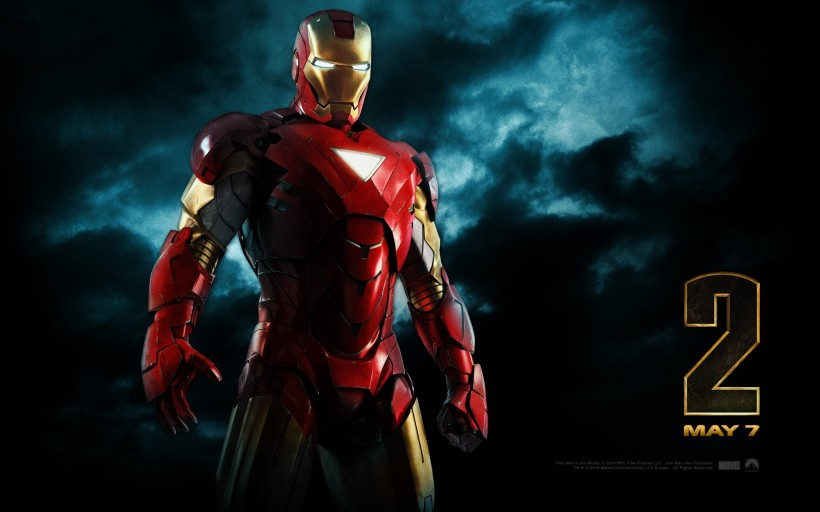
\includegraphics[width=2.5in]{./pictures/1.jpg}
		\label{label_1}
	}
	\subfloat[黑寡妇]
	{
		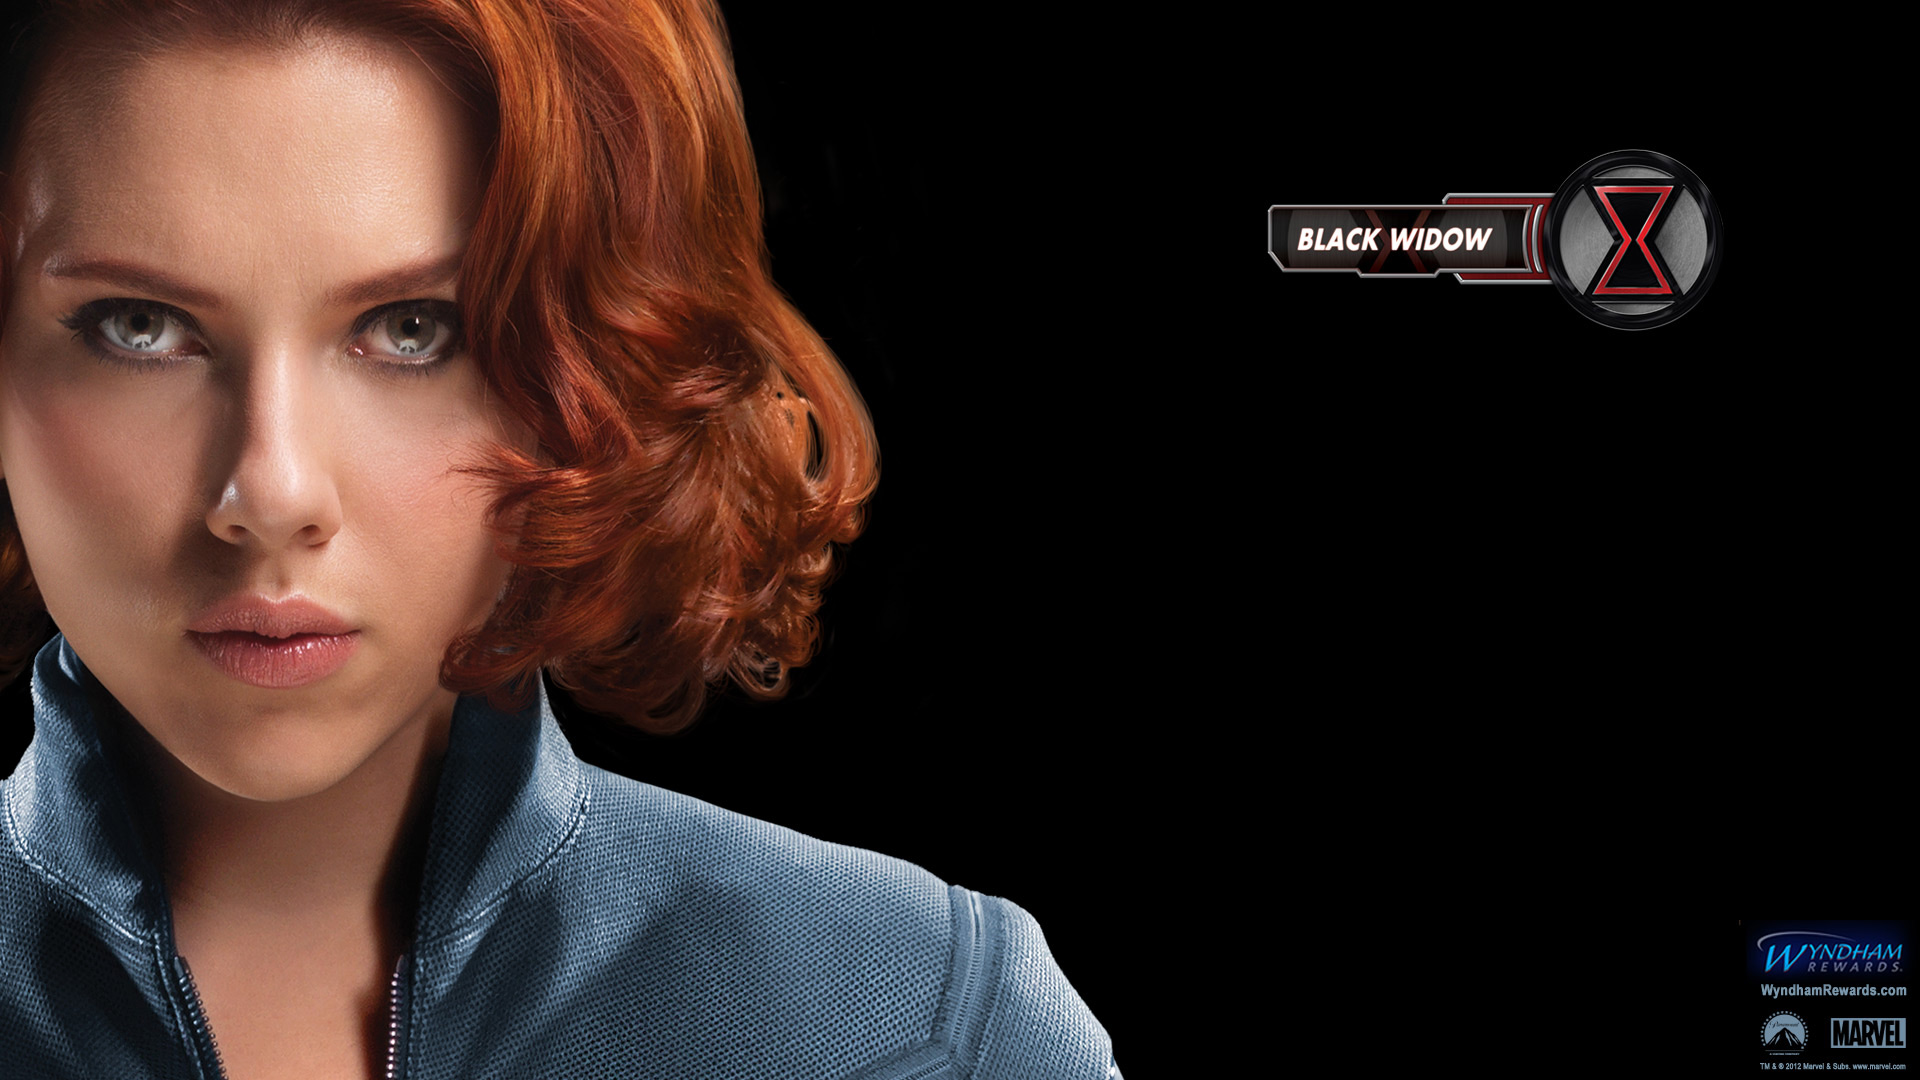
\includegraphics[width=2.5in]{./pictures/2.jpg}
		\label{labelf_2}
	}
	\quad    %用 \quad 来换行
	\subfloat[钢铁侠V]
	{
		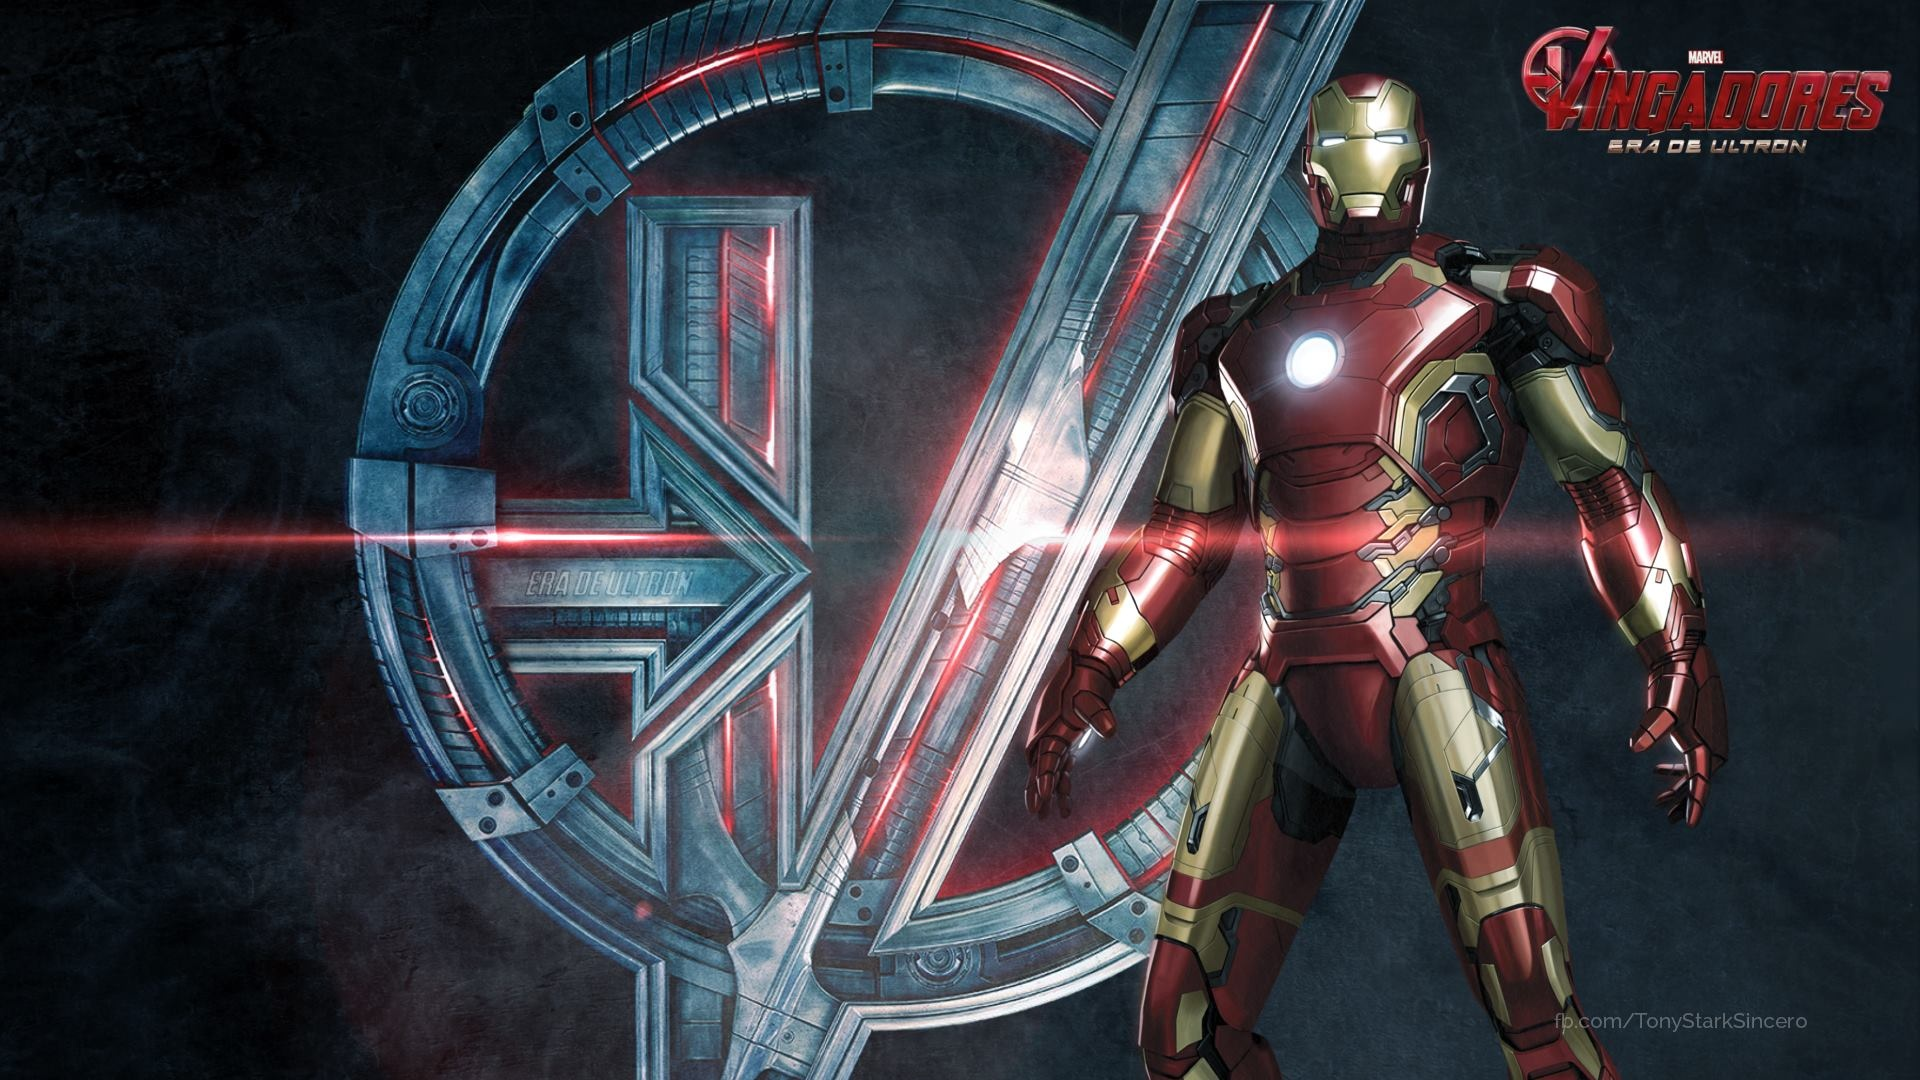
\includegraphics[width=2.5in]{./pictures/3.jpg}
		\label{label_3}
	}
	\subfloat[蝙蝠侠]
	{
		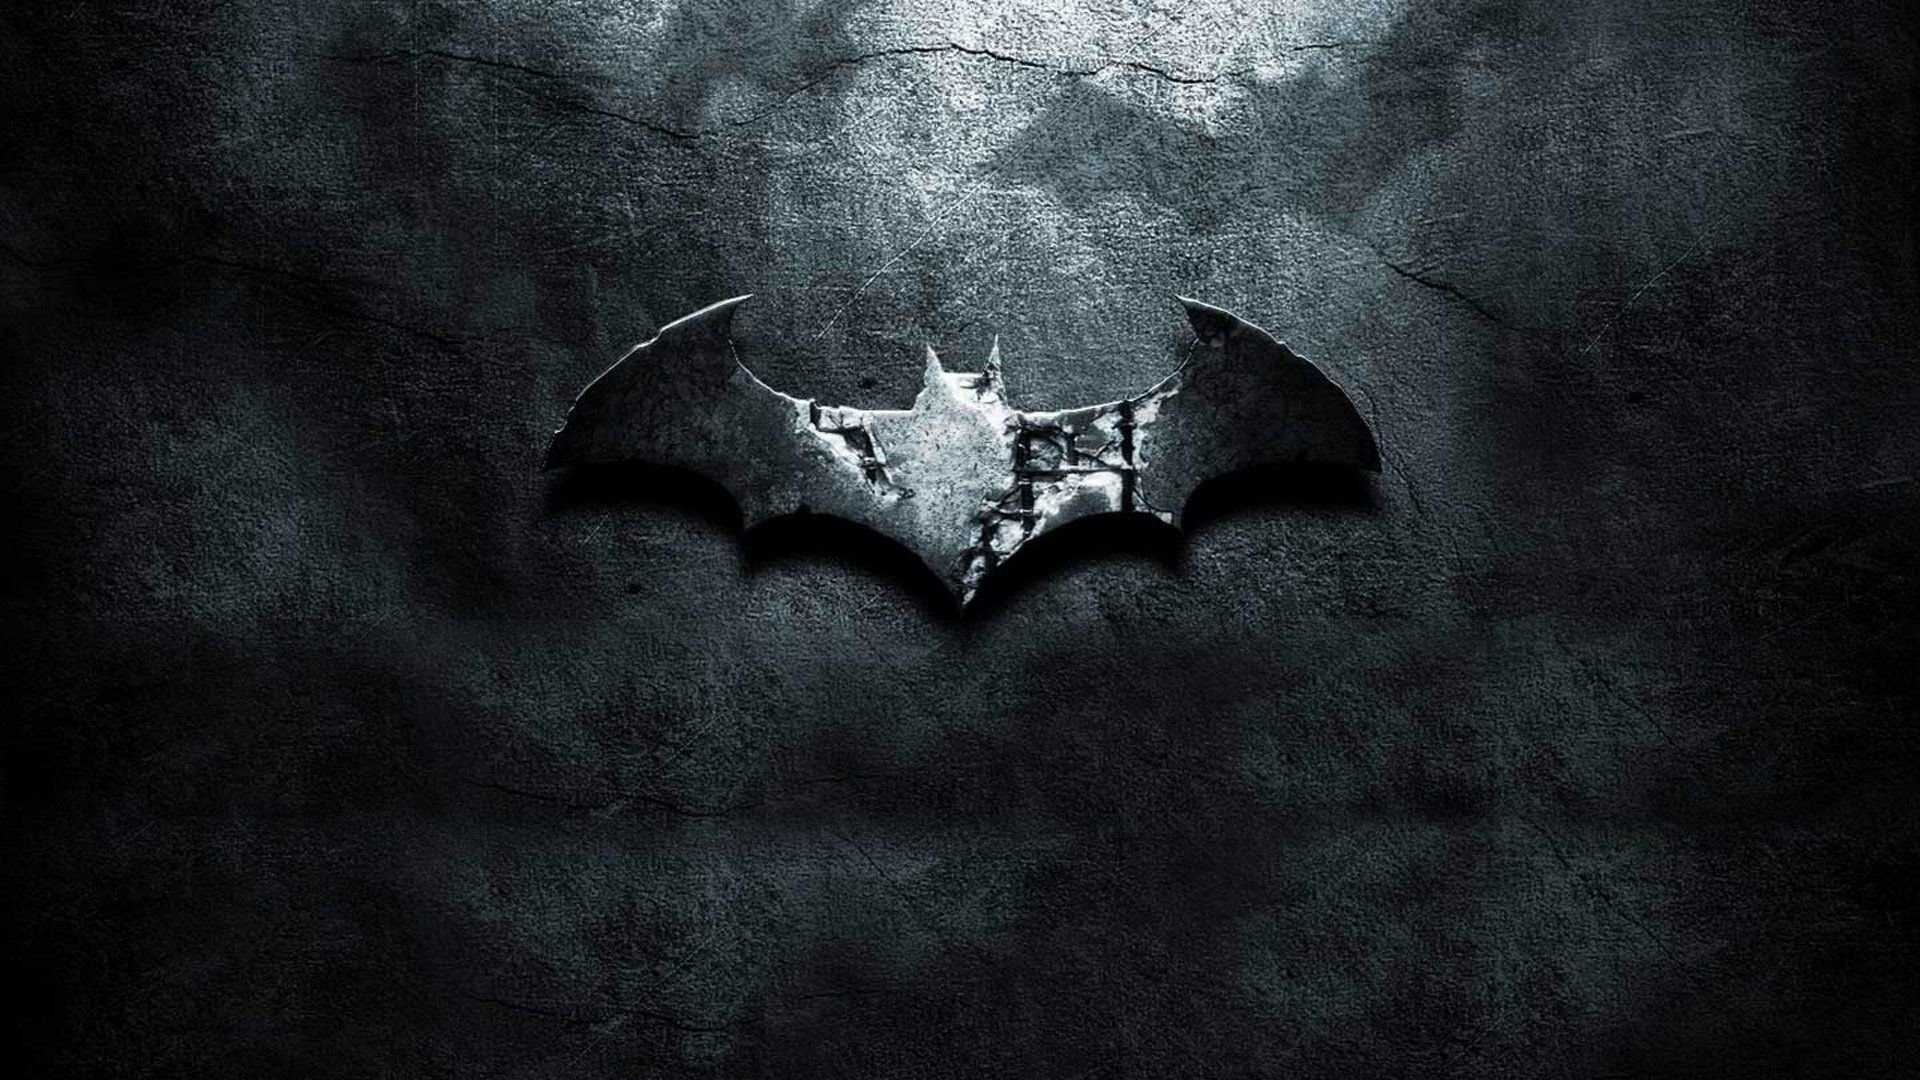
\includegraphics[width=2.5in]{./pictures/4.jpg}
		\label{label_4}
	}
	\caption{This is a Demo of $2\times 2$}
	\label{fig.1}
\end{figure}	

\end{document}
